
%------------------------------------------------------------------------------------------------
%PAGINA 21
\fancyhf{}
\fancyhead[r]{\thepage}
\begin{center}
{\fontsize{13}{16}\selectfont \textbf{SISTEMA}}
\end{center}
\vspace{0.5cm}

{\fontsize{13}{15}\selectfont
En resumen, todo estado realmente posible de un sistema $K$ es un punto en alguna región $\mathcal{S}_L(K)$ del espacio cartesiano $\mathbb{R}^n$. Véase la Figura 1.5.

\textbf{Ejemplo 1} En la teoría cinética elemental de gases, la \textbf{función de estado} es la terna compuesta por las funciones de presión, volumen y temperatura. El \textbf{espacio de estados} correspondiente es un cubo contenido en $(\mathbb{R}^+)^3$.

\textbf{Ejemplo 2} En la dinámica hamiltoniana, el \textbf{vector de estado} (o fase) es $\langle q(k, f, t), p(k, f, t) \rangle$, donde $q$ es la coordenada canónica y $p$ el momento correspondiente, ninguno de los cuales necesita ser una propiedad mecánica.

\textbf{Ejemplo 3} En la cinética química, el estado instantáneo de un sistema químico se describe por los valores de las concentraciones parciales de los reactivos y los productos de reacción. Por lo tanto, el espacio de estados del sistema es un \textbf{hipercubo} contenido en $(\mathbb{R}^+)^n$, donde $n$ es el número de componentes del sistema (reactivos, catalizadores y productos). Si hay difusión, se deben añadir ejes adicionales al espacio de estados, en particular las coordenadas de temperatura y posición.

\textbf{Ejemplo 4} En la genética de poblaciones, tres variables de estado comúnmente utilizadas son el tamaño de una población, la probabilidad (incorrectamente llamada "frecuencia") de algún gen o constelación de genes en particular, y el valor adaptativo de esta última. Por lo tanto, para un sistema compuesto por dos poblaciones que interactúan, $A$ y $B$, el espacio de estados es la región de $\mathbb{R}^6$ abarcada por los séxtuplos $\langle N_A(t), N_B(t), P_A(t), P_B(t), V_A(t), V_B(t) \rangle$ en el transcurso del tiempo.

El concepto de espacio de estados puede utilizarse para aclarar el de sistema. El espacio de estados de un \textbf{agregado} o conglomerado de cosas que no interactúan está determinado de forma única por los espacios de estados parciales. Además, dado que el

\begin{figure}[h!]
    \centering
    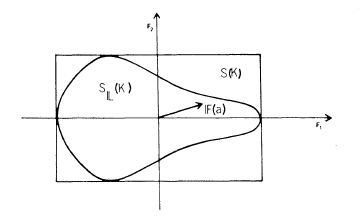
\includegraphics[width=0.6\textwidth]{imagenes/figura1.5.png}
    \caption*{Fig. 1.5. El \textbf{espacio de estados legal} $\mathcal{S}_L(K)$ de los sistemas de tipo $K$ es un subconjunto del producto cartesiano de los rangos de los componentes de la función de estado. Solo dos de esos componentes, $F_i$ y $F_j$, están representados aquí. $F(\sigma) = \langle F_i(\sigma), F_j(\sigma) \rangle$ es un estado (realmente) posible de un sistema particular del tipo dado. A medida que el tiempo 'pasa', la punta de $F(\sigma)$ se mueve dentro de $\mathcal{S}_L(K)$.}
\end{figure}
}

%------------------------------------------------------------------------------------------------
%PAGINA 22
\newpage
\fancyhf{}
\fancyhead[l]{\thepage}
\begin{center}
{\fontsize{13}{16}\selectfont \textbf{CAPÍTULO I}}
\end{center}
\vspace{0.5cm}

{\fontsize{13}{15}\selectfont
... contribuciones de esta última están todas en pie de igualdad, podemos considerar que el espacio de estados total es igual a la unión de los espacios de estados parciales. En particular, sean $\mathcal{S}_L(K)$ y $\mathcal{S}_L(M)$ los espacios de estados legales de las cosas de tipos $K$ y $M$, respectivamente. Entonces, el espacio de estados de la asociación $k+m$ de dos cosas que no interactúan de tipos $K$ y $M$ respectivamente, relativo al mismo marco de referencia, es $\mathcal{S}_L(K) \cup \mathcal{S}_L(M)$. No ocurre lo mismo en el caso de un \textbf{sistema}: aquí el estado de cada componente está determinado, al menos en parte, por los estados en los que se encuentran otros componentes del sistema, de modo que el espacio de estados total ya no es la unión de los espacios de estados parciales. Así, en el Ejemplo 4 anterior, el espacio de estados del sistema de dos componentes debe construirse \textbf{ab initio} en lugar de basarse únicamente en los espacios de estados para las biopoblaciones individuales. En resumen, una cosa es un \textbf{agregado} si y solo si su espacio de estados es igual a la unión de los espacios de estados de sus componentes; de lo contrario, es un \textbf{sistema (concreto)}. (Cf. Bunge, 1977a, 1977b.)
\\
\\Todo \textbf{evento} ocurre en o a alguna cosa concreta y consiste en un \textbf{cambio de estado} de la cosa: el cambio puede ser meramente cuantitativo, como en el caso del movimiento, o también cualitativo, como en el caso del surgimiento o la metamorfosis de una cosa. Un destello de luz, la disociación de una molécula, una tormenta, el crecimiento de un brote, el aprendizaje de un truco y la caída de un gobierno son \textbf{eventos} —o más bien \textbf{procesos}, ya que son complejos y, por lo tanto, analizables en eventos posteriores. Al ser cambios en los estados de las cosas, los eventos y procesos son representables como \textbf{trayectorias} en los espacios de estados de las cosas cambiantes. (Una cosa inmutable, si existiera, tendría un espacio de estados que consistiría en un único punto.) Diferentes trayectorias en un espacio de estados pueden tener los mismos puntos finales. Es decir, hay casos en los que una y la misma \textbf{transición neta} puede efectuarse a lo largo de rutas alternativas. Véase la Figura 1.6.
\\
\\
No se supone que las funciones $g$ y $g'$ que aparecen en la Figura 1.6 sean arbitrarias: deben ser \textbf{legales} si queremos permitir solo eventos legales y descartar los ilegales, es decir, milagros. En otras palabras, la función $g$ que aparece en la representación del evento $e = \langle s, s', g \rangle$ debe ser \textbf{compatible con las leyes} del sistema o sistemas en cuestión. Equivalentemente: un evento o proceso legal que ocurre en un sistema de tipo $K$, con puntos finales $s$ y $s'$, es representable por una terna $\langle s, s', g \rangle$, donde $g: \mathcal{S}_L(K) \rightarrow \mathcal{S}_L(K)$ es compatible con las leyes de los sistemas $K$. Si se ignoran los estados intermedios entre los puntos finales de los procesos, nos quedan flechas o pares ordenados $\langle s, s' \rangle \in \mathcal{S}_L(K) \times \mathcal{S}_L(K)$. La colección de todos estos pares de estados, es decir, el conjunto de todos los \textbf{eventos netos} (para un $g$ dado), constituye el \textbf{espacio de eventos} de los sistemas $K$ (para $g$). Símbolo:
}

%------------------------------------------------------------------------------------------------
%PAGINA 23
\newpage
\fancyhf{}
\fancyhead[r]{\thepage}
\begin{center}
{\fontsize{13}{16}\selectfont \textbf{SISTEMA}}
\end{center}
\vspace{0.5cm}

{\fontsize{13}{15}\selectfont
\begin{figure}[h!]
    \centering
    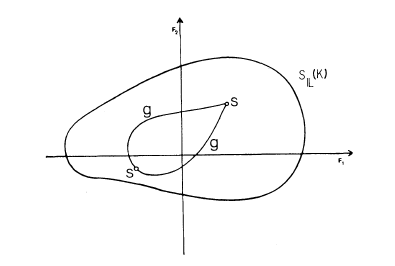
\includegraphics[width=0.6\textwidth]{imagenes/figura1.6.png}
    \caption*{Fig. 1.6. Dos procesos diferentes que resultan en el mismo cambio neto. El cambio neto del estado $s$ al estado $s'$ puede representarse como el par ordenado (o flecha) $\langle s, s' \rangle$. Dado que el cambio a lo largo de la curva $g$ puede ser distinto del cambio a lo largo de la curva $g'$, $g \neq g'$, debemos representar los eventos (o procesos) completos mediante $\langle s, s', g \rangle$ y $\langle s, s', g' \rangle$, respectivamente.}
\end{figure}
$$ \mathcal{E}(K) \subseteq \mathcal{S}_L(K) \times \mathcal{S}_L(K). $$En general, la inclusión es propia: no todas las transiciones de estado son \textbf{legales}.
\\
\\
Dado que haremos un amplio uso de la \textbf{representación del espacio de estados} en este trabajo, bien podemos comprimir lo anterior en la siguiente asunción semántica. Para cada tipo $K$ de sistema que posee $n$ propiedades, existe una función que representa propiedades $\mathbf{F}: A \longrightarrow V_1 \times V_2 \times \cdots \times V_n$ con $n$ componentes, denominada \textbf{función de estado} para sistemas de ese tipo. Además,
\\\\
(i) la \textbf{totalidad de las propiedades generales} de los sistemas de tipo $K$ es representable por el conjunto de todos los componentes (o coordenadas) de $\mathbf{F}$, es decir, $p(K) = \{F_i \mid 1 \le i \le n\}$;
\\\\
(ii) cada \textbf{propiedad particular} de un sistema de tipo $K$ es representable por un valor de un componente de $\mathbf{F}$, es decir, por $F_i(\sigma)$ para $\sigma \in A$ y algún $1 \le i \le n$;
\\\\
(iii) el \textbf{estado} de los sistemas de tipo $K$ en $\sigma \in A$ es representable por el valor de $\mathbf{F}$ en $\sigma$, es decir, $s = \mathbf{F}(\sigma) := \langle F_1(\sigma), F_2(\sigma), \ldots, F_n(\sigma) \rangle$;
\\\\
(iv) la colección de todos esos estados de cosas de tipo $K$, es decir, el rango de $\mathbf{F}$, es el \textbf{espacio de estados legal} de los sistemas $K$, o $\mathcal{S}_L(K)$ para abreviar;
\\\\
(v) todo \textbf{evento} que ocurre en un sistema de tipo $K$ es representable por una terna ordenada $\langle s, s', g \rangle$, donde $s, s' \in \mathcal{S}_L(K)$ y $g$ es un mapeo legal de $\mathcal{S}_L(K)$ en sí mismo;
\\\\
(vi) la colección de todos los eventos (legales) realmente posibles que ocurren en sistemas de tipo $K$ es el \textbf{espacio de eventos} de $K$, o $\mathcal{E}_L(K)$ para abreviar;
\\\\
(vii) para un sistema en un entorno dado, y relativo a un marco de referencia dado, la función de estado a menudo toma la forma de una función dependiente del tiempo $\mathbf{F}: \mathcal{T} \rightarrow \mathbb{R}^n$, donde $\mathcal{T} \subseteq \mathbb{R}$ es el conjunto de instantes relativos al marco dado;
\\\\
(viii) Si $\mathbf{F}: \mathcal{T} \rightarrow \mathbb{R}^n$, entonces la totalidad de los procesos que ocurren en un sistema $x$ de tipo $K$ durante el intervalo de tiempo $\tau \subseteq \mathcal{T}$ es representable por el conjunto de estados en los que se encuentra $x$ durante $\tau$:
$$ \mathbf{n}(x, \tau) = \{\mathbf{F}(t) \mid t \in \tau\}; $$
(ix) la \textbf{historia} de un sistema $x$ de tipo $K$, representable por una función de estado $\mathbf{F}: \mathcal{T} \rightarrow \mathbb{R}^n$, durante el intervalo $\tau \subseteq \mathcal{T}$, es representable por la trayectoria
$$ h(x) = \{(t, \mathbf{F}(t)) \mid t \in \tau\}; $$
(x) la \textbf{acción total} (o efecto) de una cosa $x$ sobre una cosa $y$ es igual a la diferencia entre la trayectoria forzada y la trayectoria libre del paciente $y$:
$$ \mathcal{A}(x, y) = h(y \mid x) \setminus h(y). $$
Un tratamiento detallado de estos conceptos se da en otra parte (Vol. 3, Cap. 5). A continuación, los utilizaremos para avanzar un puñado de principios generales concernientes a los sistemas.

\begin{center}
{\fontsize{13}{16}\selectfont \textbf{3. ASUNCIONES BÁSICAS}}
\end{center}

\subsection*{3.1. Cuestiones Estructurales}
Hasta ahora solo hemos hecho algunas definiciones y asunciones semánticas, pero ninguna hipótesis sustantiva sobre la naturaleza de los sistemas. (El Teorema 1.1 sobre la existencia de sistemas y la no existencia de cosas extraviadas, así como el Corolario 1.1 sobre la apertura de los sistemas, se derivaron de nuestra definición de un sistema concreto junto con ciertos postulados generales sobre la naturaleza de las cosas, establecidos en el Volumen 3.) A continuación, apostaremos por un puñado de \textbf{asunciones básicas} concernientes a los sistemas de todo tipo, siendo las primeras ciertos postulados de índole estructural. Dado que estas asunciones se referirán a las transacciones de un sistema con su entorno, bien podemos definir los conceptos de \textbf{entrada} (*input*) y de \textbf{salida} (*output*) en términos más generales de lo que hicimos en la Sec. 2.1. Comenzamos entonces con la
\\\\
\textbf{DEFINICIÓN 1.10} Sea $\sigma$ un sistema con un entorno (inmediato) $\mathcal{E}(\sigma)$. Entonces
}

}

%------------------------------------------------------------------------------------------------
%PAGINA 25
\newpage
\fancyhf{}
\fancyhead[r]{\thepage}
\begin{center}
{\fontsize{13}{16}\selectfont \textbf{SISTEMA}}
\end{center}
\vspace{0.5cm}

{\fontsize{13}{15}\selectfont
(i) la \textbf{totalidad de entradas} (*inputs*) de $\sigma$ es el conjunto de todas las acciones ambientales sobre $\sigma$:
$$ \mathbf{U}(\sigma) = \bigcup_{x \in \mathcal{E}(\sigma)} \mathcal{A}(x, \sigma); $$
(ii) la \textbf{totalidad de salidas} (*outputs*) de $\sigma$ es el conjunto de todas las acciones del sistema sobre su entorno:
$$ \mathbf{V}(\sigma) = \bigcup_{y \in \mathcal{E}(\sigma)} \mathcal{A}(\sigma, y); $$
(iii) la \textbf{actividad del entorno} de $\sigma$ es
$$ \mathcal{E}_{\mathcal{A}}(\sigma) = \bigcup_{x, y \in \mathcal{E}(\sigma)} \mathcal{A}(x, y) \cup \mathbf{U}(\sigma) \cup \mathbf{V}(\sigma). $$
Nuestra primera hipótesis es que todos los sistemas reciben entradas y son \textbf{selectivos}, es decir, aceptan solo un subconjunto (pequeño) de la totalidad de las acciones ambientales que inciden sobre ellos. Más precisamente, postulamos:

\textbf{POSTULADO 1.1} Sea $\mathbf{U}(\sigma)$ la entrada total de un sistema $\sigma$. Entonces
(i) $\mathbf{U}(\sigma) \neq \emptyset$;
(ii) $\mathbf{U}(\sigma) \subset \mathcal{E}_{\mathcal{A}}(\sigma)$ o, equivalentemente, la \textbf{función de (selección de entrada)}
$$ i: \mathbf{U}(\sigma) \longrightarrow \mathcal{E}_{\mathcal{A}}(\sigma) $$
es el mapa de inclusión (o incrustación) de $\mathbf{U}(\sigma)$ en $\mathcal{E}_{\mathcal{A}}(\sigma)$.

\textbf{Ejemplo} Hablar con las plantas es ineficaz, excepto en la medida en que las nutre con agua y dióxido de carbono.

Una segunda característica, igualmente omnipresente, de los sistemas concretos es que \textbf{reaccionan} sobre su entorno, es decir, que su salida nunca es nula. (Las llamadas \textbf{máquinas sin salida}, estudiadas en la teoría de autómatas, son, por supuesto, ficciones.) Además, en todo sistema existe actividad \textbf{espontánea}, es decir, no provocada por ninguna entrada. Así, postulamos:

\textbf{POSTULADO 1.2} Sea $\mathbf{V}(\sigma)$ la salida total de un sistema $\sigma$. Entonces
(i) $\mathbf{V}(\sigma) \neq \emptyset$;
(ii) la \textbf{función de (selección de salida)}
$$ o: \mathbf{V}(\sigma) \longrightarrow \mathcal{E}_{\mathcal{A}}(\sigma) $$
asigna a cada salida del sistema una acción ambiental, pero no a la inversa.
}

%------------------------------------------------------------------------------------------------
%PAGINA 26
\newpage
\fancyhf{}
\fancyhead[l]{\thepage}
\begin{center}
{\fontsize{13}{16}\selectfont \textbf{CAPÍTULO I}}
\end{center}
\vspace{0.5cm}

{\fontsize{13}{15}\selectfont
\textbf{Ejemplo} En toda neurona existe actividad \textbf{espontánea} que se superpone a la actividad provocada por la estimulación aferente.

Las hipótesis anteriores son principios metafísicos típicos en la medida en que pueden ser confirmados pero no refutados, pues dependen de un elemento que solo es parcialmente cognoscible, a saber, el conjunto $\mathcal{E}_{\mathcal{A}}$ de acciones ambientales. Cualquier evidencia desfavorable a nuestros postulados puede ser atribuida a nuestra ignorancia de la mayor parte de $\mathcal{E}_{\mathcal{A}}$.

La función de selección de entrada $i$ y la función de selección de salida $o$ se unen en la

\textbf{DEFINICIÓN 1.11} La función $f$ que se compone con la función de selección de salida $o$ de un sistema para producir su función de selección de entrada $i$, es decir, tal que $i = f \circ o$, se llama \textbf{función de transferencia} (o \textbf{transductora}) $f: \mathbf{U}(\sigma) \longrightarrow \mathbf{V}(\sigma)$ de $\sigma$:
\begin{figure}[h!]
    \centering
    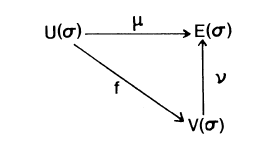
\includegraphics[width=0.4\textwidth]{imagenes/definition1.11.png}
\end{figure}

\textbf{Ejemplo} La retina transforma (o mapea o codifica) los estímulos luminosos en señales nerviosas.

Cerramos esta subsección con un conjunto de principios generales que se enunciarán de manera informal:

\textbf{POSTULADO 1.3} Sea $\sigma$ un sistema arbitrario distinto del universo. Entonces
(i) toda entrada a $\sigma$ es una salida de algún otro sistema (es decir, no hay entradas que vengan de la nada);
(ii) $\sigma$ recibe entradas de \textbf{varios tipos} (es decir, en algún momento u otro, cada uno de los componentes de la función de estado de $\sigma$ está obligado a ser afectado por cambios ambientales);
(iii) para cada acción sobre $\sigma$, existe un \textbf{umbral} por debajo del cual $\sigma$ no responde;
(iv) la entrada total de $\sigma$ tiene un componente \textbf{aleatorio} no nulo;
(v) existe un \textbf{retraso}, por pequeño que sea, entre cada entrada y la salida correspondiente, si la hay.

Hasta aquí nuestras asunciones estructurales generales. Echemos ahora un vistazo a los sistemas desde una perspectiva evolutiva.
}

%------------------------------------------------------------------------------------------------
%PAGINA 27
\newpage
\fancyhf{}
\fancyhead[r]{\thepage}
\begin{center}
{\fontsize{13}{16}\selectfont \textbf{SISTEMA}}
\end{center}
\vspace{0.5cm}

{\fontsize{13}{15}\selectfont
\subsection*{3.2. Ensamblaje y Emergencia}
Todo proceso mediante el cual un sistema se forma a partir de sus componentes se llama '\textbf{ensamblaje}'; si el proceso es espontáneo, se llama '\textbf{autoensamblaje}'. Un proceso de ensamblaje puede ocurrir en un solo paso o, más probablemente, en varios pasos: véase la Figura 1.7. Podemos expresar la idea formalmente con la ayuda del concepto de \textbf{vínculo} (*bondage*), o conjunto de enlaces entre los componentes de un sistema, introducido en la Sec. 1.2. De hecho, establecemos la
\\
\textbf{DEFINICIÓN 1.12} Sea $x$ una cosa concreta compuesta inicialmente de partes desacopladas (posiblemente sistemas en sí mismas), es decir, tal que $|\mathbf{B}(x, t)| = 0$. Entonces
(i) $x$ se ensambla en $y$ en el momento $t' > t$ si y solo si $y$ es un sistema con la misma composición que $x$ pero con un conjunto de vínculos no vacío, es decir,
$$ \mathcal{P}(y, t') = \mathcal{P}(x, t) \land |\mathbf{B}(y, t')| \ne 0; $$
(ii) el proceso de ensamblaje es de \textbf{autoensamblaje} si y solo si el agregado $x$ se convierte por sí mismo [es decir, de forma natural en lugar de artificial] en el sistema $y$;
\\
(iii) el proceso de autoensamblaje es de \textbf{autoorganización} si y solo si el sistema resultante está compuesto por subsistemas que no existían antes del inicio del proceso.

Los procesos de ensamblaje pueden ser naturales o artificiales, y los de este último tipo, a su vez, experimentales (o de laboratorio) o industriales. Los procesos de ensamblaje artificial son, por supuesto, \textbf{guiados por el hombre}. Sin embargo, hay grados de control. Una cosa es ensamblar una máquina a partir de sus partes y otra ensamblar una molécula a partir de sus precursores. En la mayoría de los casos, el último proceso
}

\begin{figure}[h!]
    \centering
    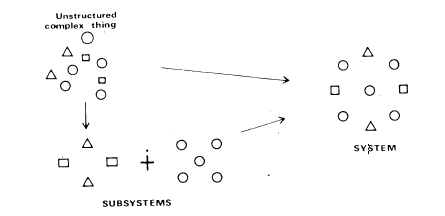
\includegraphics[width=0.7\textwidth]{imagenes/figura1.7.png}
    % Aquí se insertaría el código TikZ para la Figura 1.7
    \caption*{Fig. 1.7. Ensamblaje de un sistema a partir de unidades previamente desconectadas, ya sea directamente o por etapas.}
\end{figure}

%------------------------------------------------------------------------------------------------
%PAGINA 28
\newpage
\fancyhf{}
\fancyhead[l]{\thepage}
\begin{center}
{\fontsize{13}{16}\selectfont \textbf{CAPÍTULO I}}
\end{center}
\vspace{0.5cm}

{\fontsize{13}{15}\selectfont
... procede por sí mismo —es decir, en virtud de su \textbf{dinámica interna}— una vez que se han suministrado los reactivos y las condiciones físicas adecuadas. Por ejemplo, las proteínas e incluso las unidades ribosómicas se autoensamblan *in vitro* en cuestión de minutos si se proporcionan los precursores y las condiciones físicas adecuadas. En este caso, el hombre solo echa una mano a la naturaleza, al reproducir condiciones que han ocurrido o podrían haber ocurrido espontáneamente.

Todas las síntesis químicas y bioquímicas son, por supuesto, \textbf{procesos de ensamblaje} y, además, procesos acompañados por la \textbf{emergencia de nuevas propiedades}.

Sin embargo, el autoensamblaje ocurre en todos los niveles y de diversas maneras. Quizás el proceso de autoensamblaje más visible de todos es la \textbf{agregación} o \textbf{aglomeración} de átomos y polvo cósmico provocada por la gravitación. Se cree que así se formaron los planetas y otros cuerpos celestes. Además, lejos de conducir siempre a masas desorganizadas, la atracción gravitacional puede dar lugar a agrupaciones complejas en todas las escalas astronómicas, en particular cúmulos de estrellas, galaxias y cúmulos de galaxias. (Véase, por ejemplo, de Vaucouleurs, (1970).) Ejemplos similares de autoensamblaje por \textbf{condensación} de unidades del mismo tipo son la formación de complejos moleculares (como la polimolécula de hemocianina), de polímeros como los polipéptidos y de cristales a partir de soluciones. (Véase Calvin (1969); Eigen (1971); Lehninger (1975).) No hace falta decir que el autoensamblaje, y en particular la \textbf{autoorganización}, también ocurre a nivel social: testimonio de la formación de familias, bandas, comunidades y organizaciones sociales de diversos tipos. En resumen, el autoensamblaje y la autoorganización no son exclusivos de la vida. Lo \textbf{peculiar} de la autoorganización biótica es que resulta en \textbf{sistemas vivos} en lugar de sistemas bioquímicos o sistemas de otro tipo. (En otras palabras, es un \textbf{mecanismo de emergencia} que conduce a un nuevo nivel de organización.) Asumiremos que todos los sistemas, salvo el mundo entero, se han formado por ensamblaje:
\\\\
\textbf{POSTULADO 1.4} Todos los sistemas, excepto el universo, se originan por ensamblaje.

\textbf{Observación 1} Los sistemas naturales se originan por \textbf{autoensamblaje}, y los sistemas artificiales, por ensamblaje \textbf{artificial} o \textbf{hecho por el hombre}.

\textbf{Observación 2} Se hace una excepción para el universo porque (a) en las cosmologías naturalistas el universo no tiene origen ni fin, y (b) en las cosmologías religiosas no tiene sentido decir que el universo se origina por ensamblaje, ya que esto presupone la existencia previa de sus componentes.

\textbf{Observación 3} Ciertamente, un sistema puede formarse por la descomposición de algún supersistema. Sin embargo, esto no es un contraejemplo a nuestro postulado, que solo requiere que el sistema original
}

%------------------------------------------------------------------------------------------------
%PAGINA 29
\newpage
\fancyhf{}
\fancyhead[r]{\thepage}
\begin{center}
{\fontsize{13}{16}\selectfont \textbf{SISTEMA}}
\end{center}
\vspace{0.5cm}

{\fontsize{13}{15}\selectfont
... supersistema fue el resultado de algún proceso de ensamblaje.

\textbf{Observación 4} Nuestro axioma está lejos de ser obvio y no podría haberse formulado antes de que el \textbf{pensamiento sistémico} se volviera generalizado, aunque solo sea porque el concepto general de un sistema no había sido dilucidado hasta hace poco.

\textbf{Observación 5} Nuestro axioma es de particular relevancia para el problema del \textbf{origen de las biomoléculas y los biosistemas}. Hasta hace poco, se asumía que ambos habían sido creados por decreto divino o que habían existido desde toda la eternidad. El *Origen de las Especies* de Darwin apareció recién en 1859, y la investigación científica sobre la evolución de las moléculas comenzó solo un siglo después.

Los componentes de un sistema autoensamblado se llaman sus \textbf{precursores}, un nombre apto que sugiere que el sistema no siempre existió, sino que \textbf{emergió} de cosas preexistentes. Curiosamente, (a) los precursores de un sistema no se mezclan, sino que mantienen su individualidad hasta cierto punto, y sin embargo, (b) dan lugar a una cosa que posee \textbf{propiedades emergentes}. Por ejemplo, los dos átomos de hidrógeno que se combinan en una molécula de hidrógeno son componentes distintos de esta última, pero el \textbf{espectro} de la molécula es radicalmente diferente al de sus componentes. La primera característica se formaliza diciendo que la composición del sistema autoensamblado es igual al conjunto de las partes de sus ancestros, es decir, el conjunto de sus precursores. Y la noción de \textbf{emergencia} puede dilucidarse de la siguiente manera.

Llamemos $x$ a una cosa y $t \in \mathcal{T}$ a un instante de tiempo, e introduzcamos una función $P$ que asigna a la pareja ordenada $\langle x, t \rangle$ el conjunto $P(x, t)$ de todas las propiedades de $x$ en $t$. Es decir, $P$ es una función $P: \mathcal{T} \times \mathcal{T} \rightarrow \mathcal{P}(\mathcal{P})$, donde $\mathcal{T}$ es el conjunto de todas las cosas, $\mathcal{T}$ el conjunto de todos los instantes, y $\mathcal{P}(\mathcal{P})$ la familia de subconjuntos del conjunto $\mathcal{P}$ de todas las propiedades generales de las cosas. Un cambio en la cosa $x$ puede verse como un cierto cambio de estado de $x$. Dado que $x$ se mantiene fijo a lo largo de ese cambio de estado, podemos usar la función más simple
$$ P_x: \mathcal{T} \longrightarrow \mathcal{P}(\mathcal{P}) \text{ tal que } P_x(t) = P(x, t). $$
En resumen, $P_x(t)$ es la colección de propiedades de la cosa $x$ en el momento $t$. (Para más detalles sobre $P_x$, véase Vol. 3, Cap. 2.)

Ahora sean $t$ y $t'$ dos instantes distintos, tales que $t$ precede a $t'$. Los valores correspondientes de $P_x$ son, por supuesto, $P_x(t)$ y $P_x(t')$. Si estos dos conjuntos de propiedades de $x$ son el mismo, entonces la cosa no ha cambiado \textbf{cualitativamente}. Si son diferentes, la cosa ha ganado o perdido algunas propiedades. Si ocurre esto último, se dirá que las propiedades recién adquiridas son \textbf{emergentes} en relación con la cosa dada, aunque también puedan ser poseídas por otras cosas. En resumen, establecemos la
}

%------------------------------------------------------------------------------------------------
%PAGINA 30
\newpage
\fancyhf{}
\fancyhead[l]{\thepage}
\begin{center}
{\fontsize{13}{16}\selectfont \textbf{CAPÍTULO I}}
\end{center}
\vspace{0.5cm}

{\fontsize{13}{15}\selectfont
\textbf{DEFINICIÓN 1.13} Sea $x$ una cosa con propiedades $P(t)$ en el momento $t$, y propiedades $P(t')$ en un momento posterior $t' > t$. Entonces
(i) la \textbf{novedad cualitativa total} que ocurre en $x$ durante el intervalo $[t, t']$ es la diferencia simétrica
$$ N(t, t') = P(t) \Delta \bigcup_{\tau \le t'} P_x(\tau); $$
(ii) las \textbf{propiedades emergentes} que aparecen en $x$ durante el intervalo $[t, t']$ son aquellas en
$$ \mathcal{E}(t, t') = P(t') \setminus P(t). $$

\textbf{Ejemplo 1} Toda reacción nuclear y toda reacción química resultan en la \textbf{emergencia de cosas} dotadas de \textbf{propiedades emergentes}.

\textbf{Ejemplo 2} La descomposición (desmantelamiento) de un sistema y la sustitución de algunos de sus componentes son procesos de emergencia.

Nos atrevemos y generalizamos:

\textbf{POSTULADO 1.5} Todo proceso de ensamblaje está acompañado por la emergencia de algunas propiedades y la pérdida de otras. Es decir, sea que las partes de una cosa $x$ se autoensamblan en un sistema durante el intervalo $[t, t']$. Entonces el sistema carece de algunas de las propiedades de sus precursores —es decir, $P(t) \setminus P(t') \neq \emptyset$— pero, por otro lado, posee algunas propiedades nuevas —es decir, $P(t') \setminus P(t) \neq \emptyset$.

Hasta ahora nos hemos ocupado de la \textbf{novedad cualitativa} en una cosa particular, sin importar si las propiedades emergentes dadas son poseídas por otras cosas. Ahora dilucidamos el concepto de \textbf{emergencia por primera vez}, o \textbf{emergencia absoluta}:

\textbf{DEFINICIÓN 1.14} Las \textbf{propiedades absolutamente emergentes} (o primicias) que aparecen en una cosa $x$ durante el lapso $[t, t']$ son aquellas en
$$ \mathcal{E}_a(t, t') = \mathcal{E}(t, t') \setminus \bigcup_{y \in \mathcal{T} \setminus \{x\}} \bigcup_{\tau \le t'} P(y, \tau), $$
donde $y \neq x$ y $\tau \le t'$.

\subsection*{3.3. Selección}
Se están formando nuevos sistemas constantemente, pero no todos son \textbf{viables} en el entorno en el que emergen. De hecho, muchos son inadecuados y, por lo tanto, \textbf{efímeros}, ya sea porque son \textbf{internamente inestables} o porque \textbf{no pueden hacer frente a la agresión ambiental}. En este último caso, tenemos
}
